\clearpage
\section{Поправки к числам распадов $\Lb$}
\label{sec:corrections}

Задача алгоритма аппроксимации -- найти такую точку в многомерном 
пространстве параметров, для которой определенная функция, выражающая 
близость модели к изучаемому спектру, достигает экстремального значения. 
Проблема минимизации во многих измерениях нетривиальна, а требования 
к скорости и эффективности работы еще больше усложняют алгоритм. В таких 
условиях при наличии большого числа параметров и сложной зависимости 
модели от них повышается вероятность появления искажений, обусловленных 
неточностью алгоритма. Предугадать и оценить их чрезвычайно сложно, 
и поэтому необходимо выполнять проверки в каждом случае индивидуально. 
Проводить такое исследование для каждой аппроксимации нецелесообразно, 
но одним из конечных этапов анализа необходимо рассмотреть критически 
важные и подверженные искажениям результаты и при необходимости внести 
соответствующие поправки.
%
Работа по изучению очарованных резонансов в распаде 
$\Lb\to\Lc\pip\pim\pim$ далека от завершения, и проверка на искажение 
результата в ней еще не проводилась. Работа же по измерению распадов 
$\Lb\to\Doptstarp\p\pim\pim$ уже завершена 
и опубликована~\cite{lb2dppipi-paper}. Подверженным искажениям этапом 
анализа является извлечение чисел событий распадов 
$\Lb\to\Dp\p\pim\pim$, $\Lb\to\Dstarp\p\pim\pim$, 
$\Lb\to\Lc\pip\pim\pim$ при аппроксимации экспериментальных спектров 
инвариантных масс $m(\Dp\p\pim\pim)$ и $m(\Lc\pip\pim\pim)$. Эти 
результаты были приведены в разделе~\ref{sec:fitting:lb-dppipi} 
в таблице~\ref{tab:lb-fit-results}. Для оценки имеющихся в них возможных 
искажений проводилась следующая процедура, описанная далее.

Поскольку взаимодействие протонов при соударении, рождение кварков, их 
адронизация и распад, а также регистрация конечных заряженных частиц 
детектором и восстановление событий происходят по вероятностным законам, 
а экспериментальные спектры строятся на основе этих данных, сами 
спектры, хоть и имеют определенные фиксированные свойства, но являются 
случайными по своей природе. Вследствие этого, любые результаты, 
извлекаемые из спектров, тоже являются случайными величинами. Таким 
образом, итогом аппроксимации является не единственная точка 
в пространстве параметров, а некая область, которую чаще всего 
представляют $n$\nobreakdash-мерным кубом. Размеры области зависят от 
объемов доступных для аппроксимации данных, а искажения проявляются 
ввиду конечности числа событий в экспериментальном спектре.
%
Для исследования корректности извлекаемых результатов необходимо 
обработать статистически значимый набор спектров, аналогичных 
экспериментальному, и проследить за изменениями интересующих параметров. 
Создание аналогичных экспериментальному спектров производится с помощью 
модели, полученной в результате его аппроксимации. Модель представляет 
собой функцию распределения вероятностей, на основе которой можно 
создать набор значений случайной величины, инвариантной массы, 
отличающийся от экспериментального в пределах статистических 
погрешностей. Необходимо также учесть, что полное число 
зарегистрированных детектором событий тоже является случайным, а значит 
подлежит вариации при генерации каждого конкретного набора.

На основе модели, полученной в результате аппроксимации 
экспериментальных спектров инвариантных масс, создавались так называемые 
псевдоэксперименты, которые затем аппроксимировались этой же моделью. 
Для интересующих параметров результаты аппроксимации записывались в виде 
нормированных на найденную погрешность отклонений от экспериментального 
значения:
\[ x_p = (p^\text{fit} - p^\text{data}) / \sigma_p^\text{fit}, \]
где $p^\text{fit}$ и $\sigma_p^\text{fit}$ -- значение и погрешность 
параметра $p$, полученные в результате аппроксимации псевдоэксперимента, 
а $p^\text{data}$ -- величина параметра, определенная из 
экспериментальных данных. Среднее значение и дисперсия такого 
отклонения, вычисленные на основе статистически значимого количества 
созданных на основе модели спектров, отражают вносимые алгоритмом 
минимизации искажения. Если они отличаются от нуля и единицы, 
соответственно, необходимо ввести поправку, компенсирующую неточность 
алгоритма. Обозначая за $\mu_p^x$ и $\sigma_p^x$ среднее значение 
и дисперсию отклонения $x_p$ параметра $p$, можно сказать, что алгоритм 
аппроксимации смещает значение параметра на $\mu_p^x$ стандартных 
отклонений, а погрешность недооценивает или переоценивает в $\sigma_p^x$ 
раз. Корректировка результата аппроксимации для параметра $p$ в таком 
случае выглядит следующим образом:
\[ p^\text{corr} = p^\text{data} + \mu_p^x\,\sigma_p^x\,\sigma_p^\text{data},
\qquad \sigma_p^\text{corr} = \sigma_p^x\,\sigma_p^\text{data}. \]

Проверка на наличие искажений была проведена для чисел событий, 
соответствующих вкладам распадов $\Lb\to\Doptstarp\p\pim\pim$ 
и $\Lb\to\Lc\pip\pim\pim$ в спектрах масс $m(\Dp\p\pim\pim)$ 
и $m(\Lc\pip\pim\pim)$, соответственно. Распределения нормированных 
отклонений для них приведены на рисунке~\ref{fig:pulls}, 
а соответствующие поправки вычислены в таблице~\ref{tab:pulls}.
%
\begin{figure}[t!]%pulls{{{
  \centering
  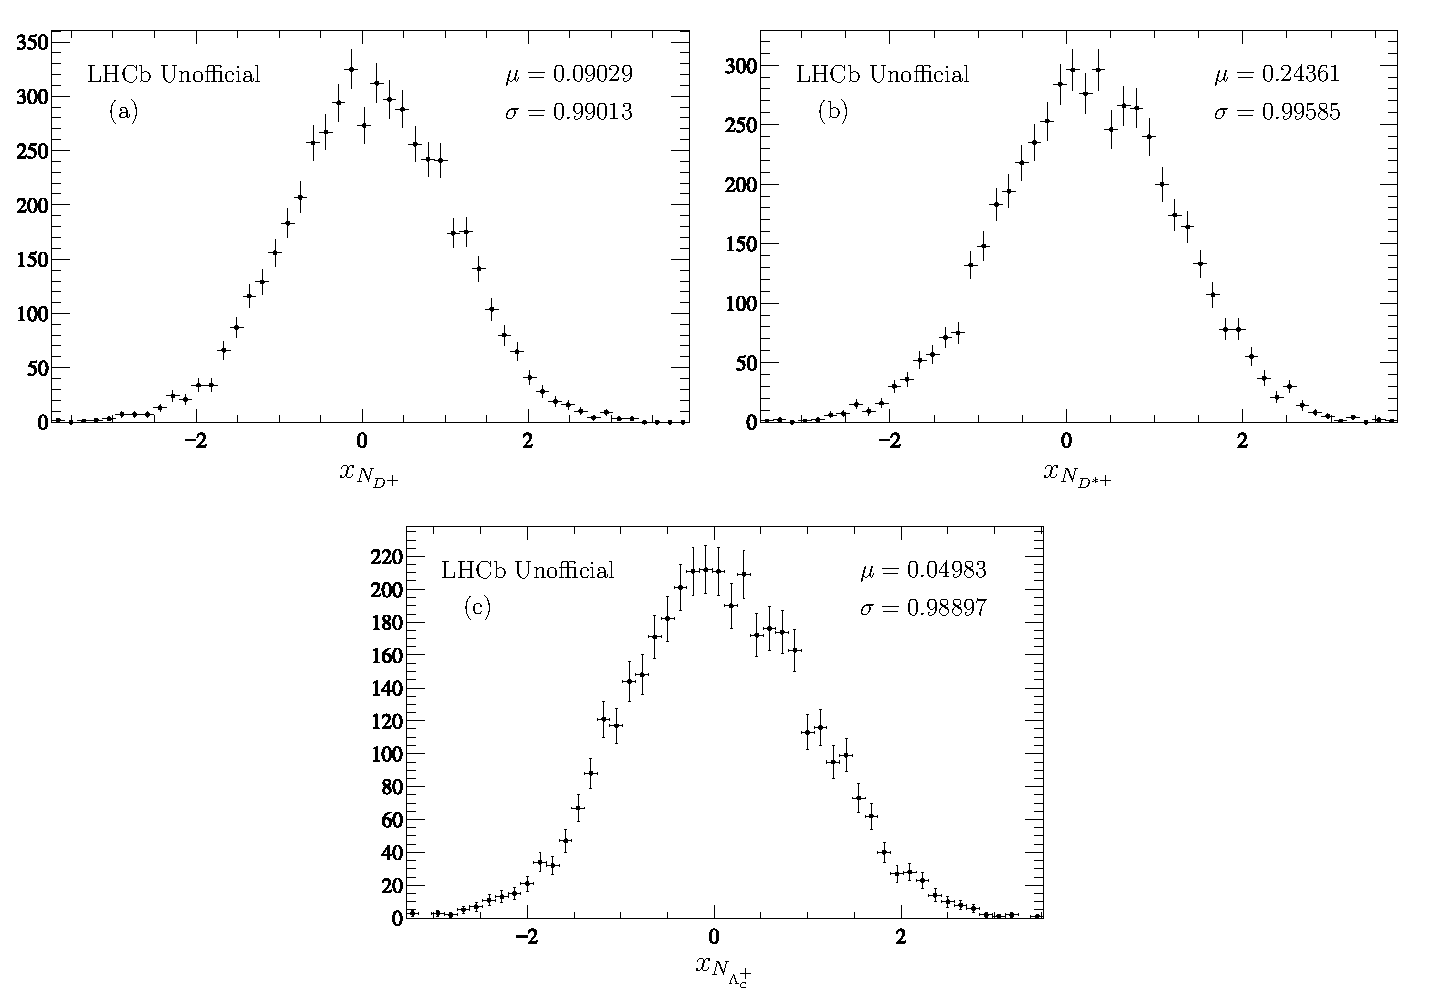
\includegraphics[width=\linewidth]{figures/toy-pulls}
  \caption{Распределения относительных отклонений количеств распадов 
  $\Lb\to\Dp\p\pim\pim$~(a), $\Lb\to\Dstarp\p\pim\pim$~(b) 
  и $\Lb\to\Lc\pip\pim\pim$~(c) от значений, извлеченных из 
  экспериментальных данных, полученные при аппроксимации 
  псевдоэкспериментов.}
  \label{fig:pulls}
\end{figure}%}}}
%
\begin{table}%pulls{{{
  \centering
  \caption{Поправки к количествам распадов $\Lb\to\Dp\p\pim\pim$, 
  $\Lb\to\Dstarp\p\pim\pim$, $\Lb\to\Lc\pip\pim\pim$, извлеченным из 
  экспериментальных данных, обусловленные алгоритмом аппроксимации.}
  \label{tab:pulls}
  \begin{tabular}{|c | r|l | c|c | r|l|}
    \hline
    Параметр & $N^\text{data}$ & $\sigma_N^\text{data}$
             & $\mu$ & $\sigma$
             & $N^\text{corr}$ & $\sigma_N^\text{corr}$ \\
    \hline
    $N_\Dp$    & 1933 & $\pm56$ & 0.090 & 0.990 & 1938 & $\pm55$ \\
    $N_\Dstarp$ & 862 & $\pm55$ & 0.244 & 0.996 &  875 & $\pm55$ \\
    $N_\Lc$  & 26505 & $\pm177$ & 0.050 & 0.989 &26515 & $\pm175$ \\
    \hline
  \end{tabular}
\end{table}%}}}
%
Как видно, искажениям в результате аппроксимации оказалось подвержено 
только число распадов $\Lb\to\Dstarp\p\pim\pim$, а поправки к остальным 
величинам учитывать было бы некорректно, поскольку они меньше 
погрешностей, обусловленных конечностью числа проведенных 
псевдоэкспериментов. Погрешности чисел распадов алгоритм аппроксимации 
оценивает точно.

Помимо искажений, вносимых алгоритмом аппроксимации, необходимо учесть 
наличие еще нескольких явлений, приводящих к отличию полученных значений 
от настоящих чисел распадов $\Lb\to\Doptstarp\p\pim\pim$, 
$\Lb\to\Lc\pip\pim\pim$.
%
Во-первых, поскольку очарованные адроны регистрируются в модах 
$\Dp\to\Km\pip\pip$, $\Lc\to\p\Km\pip$, конечные частицы, регистрируемые 
детектором, одинаковы для всех трех распадов. Это приводит к возможности 
перекрестного вклада одних событий в другие, поскольку процедура 
восстановления треков частиц и нахождения вершин распадов может ошибочно 
составить, например, $\Dp$ из частиц $\Km\pip\pip$, образованных на 
самом деле в распаде $\Lb\to\Lc(\to\p\Km\pip)\pip\pim\pim$. Вклад 
распадов через $\Lc$ в область непосредственно под пиком распада через 
$\Dp$ значителен и требует учета. Вклад же в область под распадом через 
$\Dstarp$ невелик, поскольку она существенно удалена от пика $\Lb$, 
в котором находится подавляющее большинство распадов через $\Lc$. 
Обратный вклад распадов $\Lb\to\Doptstarp\p\pim\pim$ под пик $\Lb$ 
в спектре инвариантных масс $m(\Lc\pip\pim\pim)$ мал и не требует учета, 
поскольку интегральное число событий во вкладах $\Doptstarp$ на порядок 
меньше количества зарегистрированных распадов $\Lb\to\Lc\pip\pim\pim$.
%
Во-вторых, наряду с распадом $\Lb\to\Lc\pip\pim\pim$, в котором 
присутствует множество подканалов, идущих по сильному взаимодействию, 
присутствует распад $\Lb\to\Lc\Dsubsm$, в котором $\Dsubsm$ распадается 
на три пиона по слабому взаимодействию.
%
В-третьих, некоторые события с распадами $\Lb\to\Lc\pip\pim\pim$, ввиду 
особенностей работы алгоритмов восстановления треков, учитываются 
дважды. Это происходит, если два положительных пиона в конечном 
состоянии, один из которых образован напрямую при распаде $\Lb$, 
а другой появляется при распаде $\Lc$, с точки зрения накладываемых для 
отбора событий ограничений, могут обменяться своими ролями и все равно 
составлять необходимые вершины распадов адронов.
%
Для учета трех описанных явлений необходимо ввести соответствующие 
поправки к найденным на предыдущих этапах количествам событий. Это не 
было частью данной работы, и поэтому весь процесс детально не 
описывается. Однако поправки необходимы для получения отношений 
вероятностей исследуемых распадов $\Lb$. По результатам поправок числа 
событий становятся равны $N_\Dp = 1542\pm60$, $N_\Lc = 25910 \pm 180$.

Кроме того, отношения полученных чисел нельзя напрямую приравнивать 
к отношениям вероятностей распадов, поскольку используемые для отбора 
событий критерии могут по-разному сказываться на распадах. Для каждого 
распада на основе моделирования и дополнительных наборов 
экспериментальных данных определяется доля событий, проходящих как 
триггер детектора, так и отбор, используемый в анализе для подавления 
фона. Эти доли называются эффективностями, а для дальнейшей работы 
используются их отношения. Именно неточности определения эффективностей 
зачастую вносят ощутимый вклад в погрешности извлекаемых величин, 
а выбор используемых каналов распада очарованных адронов обусловлен 
именно стремлением минимизировать их влияние. Нахождение эффективностей 
также не являлось частью данной работы, но необходимо для получения 
конечных результатов. Их отношения оказались равны
\[ \eps^\text{tot}_\Dp / \eps^\text{tot}_\Lc = 1.112 \pm 0.009, \quad
\eps^\text{tot}_\Dstarp / \eps^\text{tot}_\Dp = 0.926 \pm 0.008,\]
где неопределенности обусловлены конечностью используемых для вычисления 
эффективностей наборов данных.
